\subsection{Design Considerations}\label{sub_sub_section:tgt_intra_comms_design_considerations}

\subsubsection{Modularity}\label{sub_sub_section:tgt_modularity}
\paragraph{Relevance}
Mechanical modularity is the most obvious path as the components need to physically connect easily. However, the communication architecture also needs to support this so that devices can easily communicate even if they are changed completely.
\paragraph{Modular Communication Protocols}
Defined interfaces, protocols and pin allow for different devices to communicate without specific dependencies on each other with protocols such as those in \ref{tab:communication_options}. Therefore, integrating new sensors or modules does not require a new communication system. Another key property of modular networks is physical, some networks lend themselves better to modular design, for example for a \gls{CAN} Bus you only need to add a stub.

\subsubsection{Telemetry}\label{sub_sub_section:tgt_telemetry}
\paragraph{Battery Telemetry}
The two key failure modes for the battery are state of charge and thermal runaway. Both can cause complete failure and therefore both should be monitored during flight. This allows for \gls{RTH} to be triggered in case of a state of charge or emergency landing in the case of thermal runaway.
\paragraph{\gls{ESC} Telemetry}
\gls{IMU} data can be used in conjunction with command signals to approximate actuator faults, however, due to noise and outside disturbances it is limited in accuracy. Providing \gls{ESC} telemetry for voltage, current and \gls{RPM} is important information when classifying motor and propeller faults accurately used in \ref{para:control_strategy}.   

\subsubsection{Redundancy and Safety Critical Devices}\label{sub_sub_section:tgt_redundancy}
\paragraph{Relevance}
Safety critical devices ensure that the drone does not sustain damage or isolate itself. This includes components necessary for flight and the sensors required for \gls{RTS}. To ensure that failures are minimised, safety critical devices should be redundant. If a safety critical device does not have a redundant version it should be able to communicate on at least two different lines preventing a single module failure causing device failure.
\paragraph{Node Distribution}
Distributing the devices on different communication lines reduces the risk of failure as it reduces the risk of common mode failure. For example, if a \gls{GNSS} module were to have an improper fixture and move in a way that it severs all connections; if both communication lines are in it, both are severed. However, if it is on only one communication line then the other communication line is undamaged. This layout is shown in \ref{fig:CAN_bus}. The major drawback is that it leaves the system more vulnerable to dual failures as if the primary bus breaks and the redundant module is not functional the working primary module cannot be used by the redundant bus highlighting the importance of regularly testing the redundant modules and lines even if unused.
 \begin{figure}[h!]
 \centering
  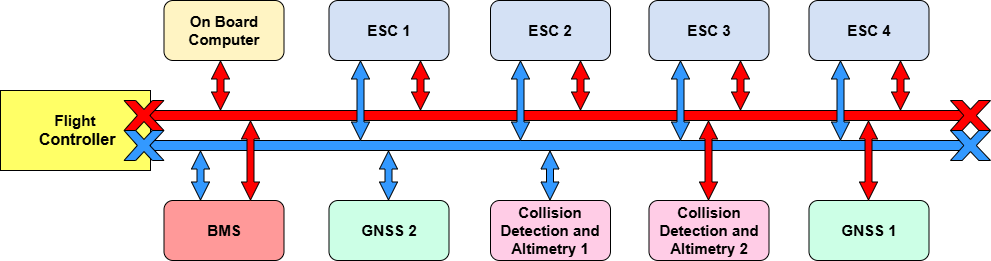
\includegraphics[width=1\textwidth]{figs/Thomas/Intra Communication/CAN bus.png}
 \caption{Bus layout}
 \label{fig:CAN_bus}
 \end{figure}